
\subsection{Types and Functions}

In the LHC, there are various accelerator magnets which can be divided into three main groups based on their function~\cite{cern_main_webpage}: 
\begin{enumerate}
    \item Main dipole magnets. They bend the moving particles in order to keep them in the trajectory of a 27 km-long ring of the LHC. There are 1232 dipoles in the LHC.
    \item Main quadrupole magnets. They constrain the width and the height of a particle beam in order to maintain it inside of the vacuum chamber within the LHC magnet. There are 392 such magnets inside the LHC.
    \item Corrector magnets. One of their goals is to correct imperfections in the field quality created in the aforementioned magnets. Some of the examples of such magnets are: quadrupoles and skew quadrupoles, sextu-, octu-, deca- or dodecapoles. 
\end{enumerate}

Figure~\ref{fig:cross_section_lhc_main_dipole} presents the cross-section of the main LHC dipole. The particle beam is travelling inside of a beam pipe surrounded by a double-layer coil composed of multiple turns of a~superconducting cable. The coils are clamped with pre-stressed steel collars in order to oppose the Lorentz forces acting on them during the machine operation. Since the magnets are mounted at room temperature, the pre-stress also serves for maintaining the elements position when the entire structure shrinks during the cooling process. In principle, the pre-stress maintains the contact between the coil and neighbouring elements which allows for avoiding friction and, thus, the heat generation. The collars are surrounded by a concentrically mounted iron yoke. The iron yoke increases the central magnetic field that directs the~travelling beam.

\begin{figure}[H]
    \centering
    \begin{tikzpicture}
    \node at (0,0) {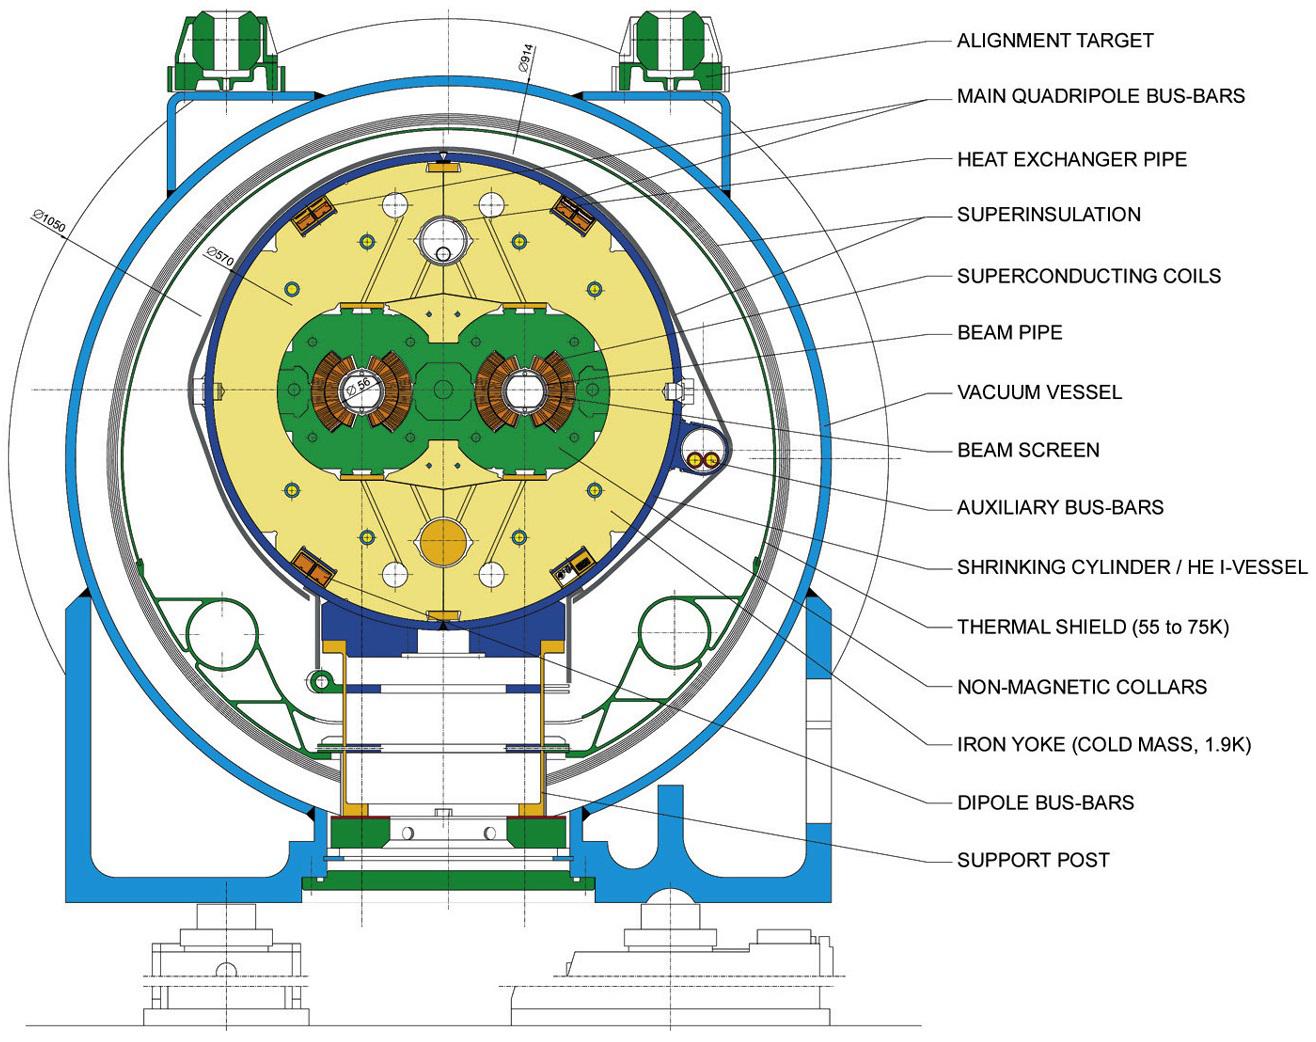
\includegraphics[width=.75\textwidth]{sections/introduction/figures/LHC_main_dipole_cross_section.png}};
    \end{tikzpicture}
    \caption{Cross-section of the LHC main dipole magnet with description of main components~\cite{lhc_main_dipole_cross_section}.}
    \label{fig:cross_section_lhc_main_dipole}
\end{figure}

\subsection{Quench Protection}

When a quench occurs during the operation of a superconducting magnet, it~must be detected in the shortest possible time. As soon as the quench is detected, the~power converter, that supplies with current magnets connected in series, is switched off and energy, mostly magnetic, stored in the circuit is discharged. In principle, the energy should be either deposited in the coil or extracted from the magnet. The quench protection systems can be passive or active. The passive systems do not use any additional electronics which triggers the quench protection devices. An example of a passive protection system is a diode connected in parallel to a~magnet. When the quench occurs, both the diode and the magnet are subjected to the same resistive voltage. If the resistive voltage reaches the forward diode voltage, the diode allows the current to bypass the magnet.

Among others, three active protection systems are described: 

\begin{enumerate}
    \item Quench heaters
	\item Coupling-Loss Induced Quench (CLIQ) system
	\item Energy extraction
\end{enumerate}

Quench heaters are resistive strips installed along the coils in close contact with the~windings. The heaters have an external power supply usually based on a charged capacitor. When a quench is detected, the heaters are fired. Due to the firing of the protection system, the quench heater spots, being in close contact with the windings, quench inside of a coil. This process supports the longitudinal quench propagation initiated at each of the quench heater spots. A~larger resistive volume is created in the magnet and the current discharge occurs more quickly. The quench heaters have an external power supply independent of the superconducting coils. Therefore, they must be electrically insulated from the windings. In fact, the electrical insulation is a thermal barrier causing a~delay between the moment when the heaters are fired and the time when the coil quenches. This delay is a characteristic feature of a quench heater system. The~drawbacks of the quench heaters are as follows~\cite{salmiquenchheateroptimization}: 

\begin{enumerate}
    \item On one hand, the quench heater system requires a high thermal diffusivity, i.e. the~insulation between the heater and the coil should be thin enough to decrease the delay of the firing system. Meanwhile, the system should meet the requirements of an electrical insulator, which should be thick enough to prevent short-circuits. These two requirements are contradictory with respect to one another. 
	\item There is no possibility to replace quench heating strips of the magnet once they are installed. Therefore, in case a failure during the machine operation, the maintenance of this system is limited in a~long-term. 
\end{enumerate}

In addition, there exists a natural effect that enables a magnet to discharge quicker, called a “quench back”. According to the Faraday’s law, the variation of a magnetic field in time induces eddy currents in an electrical conductor. The heat generated due to this phenomenon is referred as AC-losses. If the current drops sufficiently quickly, the AC-losses may induce a quench in the parts of a coil which remain superconducting. The CLIQ system is based on the same physical principle. It generates current oscillations in the superconducting windings to create a fast change of the magnetic field. According to~\cite{ravaioli_cliq_phd_thesis}, the CLIQ protection is more efficient with respect to the quench heaters in the operating conditions of a magnet close to the critical surface. CLIQ is implemented as a baseline for the inner triplets\footnote{Inner triplets provide the final focusing of the proton beams at four collision points of the LHC~\cite{lhc_inner_triplet_powering_strategy}.} for the HL-LHC project.

In the energy extraction system, a dump resistor is connected in series to a set of superconducting magnets in a circuit. When the~quench is detected, an active switch allowing the current to bypass the dump resistor is disconnected.  Thus, a~part of the energy stored in the circuit is discharged in the resistor. This system allows for a faster recovery of a magnet to its operating conditions because it requires less cooling power after the discharge process.~\cite{salmiquenchheateroptimization}

A superconducting magnet can also be "self-protected" meaning that the energy accumulated in the circuit is discharged by a natural rise of resistivity inside of the magnet. This is the simplest and most cost-effective solution. The self-protectability is applicable in magnets characterised by relatively low current densities and, therefore, low magnetic fields. A~relatively small amount of discharged energy in these magnets allows for limiting the temperature rise during the quench. In principle, the self-protectability should be the baseline for the magnet protection. However, if the energy density is too high, one should opt for an additional protection equipment.

\subsection{Magnet Design Key Parameters}

From the magnet design standpoint, the key parameters are:
\begin{enumerate}
    \item peak voltage to ground
    \item maximum hot-spot temperature
\end{enumerate}

Temperature is rarely measured in experiments because there is no space to mount temperature sensors within the magnets. It is physically deduced from the resistive voltage measured across the magnet as a quench propagates. The place where a quench starts propagating is characterised by the highest temperature in the entire magnet during quench (also referred as the hot-spot temperature). The rise of resistive voltage inside the magnet must also remain within the allowable voltage-to-ground limits as well as turn-to-turn voltage limits imposed by electrical properties of the insulation. Exceeding these limits may lead to:

\begin{enumerate}
    \item Short-circuit between different windings of the coil across the internal windings' insulation,
    \item Short-circuit between the winding and the ground across the ground insulation of the magnet.
\end{enumerate}

The hot-spot temperature and the voltage-to-ground value allow for defining whether the materials reach their safety limits at which they loose mechanical, thermal or electro-magnetic properties leading to the magnet destruction. Therefore, there is a need to study the evolution of the key parameters in the process of a magnet design when the quench occurs in the considered system.